% !TeX root = diploma.tex

\chapter{Применение $\sn$-модели к собственному одноосному сегнетоэлектрику Sn$_2$P$_2$Se$_6$}\label{ch:appl}

\section{Введение}\label{sec:applintro}
В данном разделе рассматриваются свойства НСФ в одноосном собственном СЭ Sn$_2$P$_2$Se$_6$.
Это вещество принадлежит к семейству твердых растворов (Pb$_y$Sn$_{1-y}$)$_2$P$_2$(Se$_x$S$_{1-x}$)$_6$, имеющих однокомпонентный ПП (спонтанная поляризация, ориентированная вдоль некоторой оси) \cite{Vysochanskii1994}. 
Сегнетоэлектрик-полупроводник Sn$_2$P$_2$Se$_6$ является весьма перспективным для использования в технике как рабочая среда в тепловых и акустических приемниках, однако при этом данное вещество теоретически исследовано пока недостаточно \cite{Vysochanskii1994}. 

Существующие в настоящее время теоретические подходы не позволяют корректно интерпретировать целый ряд обнаруженных в последние годы свойств данных веществ. 
Так, для одноосных собственных СЭ обнаружена «аномальное» с точки зрения предыдущих представлений поведение ряда характеристик (пространственного распределения ПП, температурной зависимости волнового вектора, скачка теплоемкости, интегральной интенсивности сателлитов в дифракционных экспериментах, диэлектрической восприимчивости и т.д.) вблизи точки фазового перехода в СФ. 

В связи с этим актуальны следующие исследования поведения несоразмерных структур ПП вблизи точек фазовых переходов, особенно перехода в СФ, а также описание НСФ в конкретных веществах, в частности в одноосных собственных СЭ семейства твердых растворов (Pb$_y$Sn$_{1-y}$)$_2$P$_2$(Se$_x$S$_{1-x}$)$_6$, имеющих однокомпонентный ПП.

Равновесные распределения ПП $\varphi(x)$ в одноосных собственных СЭ, как правило, близки к синусоидальным даже вблизи точки перехода в СФ. 
Так, в нитрите натрия NaNO$_2$ отношение амплитуды третьей гармоники $a_3$ к амплитуде фундаментальной $a_1$ (т. е. первой) не превышает 0.03 \cite{Ema1990}.

Предложенные в настоящее время модификации одногармонической модели (учет нескольких высших гармоник, описание вклада упругих сил и др.) позволили частично улучшить описание несоразмерной фазы в некоторых системах с однокомпонентным ПП (например, для нитрита натрия обзор этих результатов дан в  работе \cite{Ema1990}). Однако эти рекомендации не носят универсальный характер и не применимы в полном объеме, например, к тиомочевине, для которой вклад высших гармоник волны модуляции ПП относительно велик (отношение амплитуды третьей гармоники к амплитуде первой гармоники составляет около 0.1).

Вместе с тем, поведение одноосных собственных СЭ не удается адекватно описать в рамках до сих пор применявшегося одногармонического приближения, когда распределение ПП в НСФ аппроксимируется согласно
\begin{equation}
\varphi(x) = a \cdot \sin(bx)
\label{eq:sinmodel}
\end{equation}

Так, для Sn$_2$P$_2$Se$_6$ детальный термодинамический анализ показал \cite{Khoma1998}, что, несмотря на относительно малый вклад высших гармоник в структуру волны модуляции \cite{Barsamian1993}, корректно воспроизвести ряд важнейших свойств НСФ в рамках модели \eqref{eq:sinmodel} не удается. 
Например, зависимость волнового вектора $k$ модуляции ПП от температуры в модели \eqref{eq:sinmodel} имеет кривизну, противоположную наблюдаемой в эксперименте (см. рис. 10 в \cite{Khoma1998}). 
Кроме того, необходимость включения высших гармоник следует из сравнения теоретических расчетов $\Delta C_p$ с экспериментальными данными \cite{Khoma1998}.

Из изложенного выше следует необходимость разработки новых подходов для описания НСФ в разнообразных веществах и, в частности, в Sn$_2$P$_2$Se$_6$, описывающих нелинейные свойства и температурную эволюцию пространственно-неоднородных состояний во всем интервале существования НСФ. 
Принципиально важным этапом является отбор физически значимых распределений и детальное выяснение возможности их применения для описания равновесного и метастабильных состояний системы, распределения ПП в критических зародышах новой (соразмерной) фазы, а также состояний, реализующихся в области фазового перехода. 
Предварительный анализ, проведенный \cite{Barsamian1993}, показывает, что к особенно перспективных в этом отношении распределений ПП относятся зависимости, которые выражаются через эллиптические функции Якоби и гиперэллиптические функции, параметры которых определяются путем минимизации ТП.

Все рассматривавшиеся ранее модели таких структур основывались на учете конечного числа Фурье-компонент разложения ПП. 
В этой работе сделана попытка объяснить некоторые свойства НСФ путем рассмотрения в качестве модельного решения вариационного уравнения эллиптическую функцию Якоби $\sn$, что фактически позволяет ``учесть'' сразу все гармоники Фурье-разложения ПП. 
Модель, формально учитывающая бесконечное число гармоник волны модуляции ПП $\varphi(x)$, была предложена в \cite{Berezovsky1998}.

\section{Сравнение одногармонической и sn моделей}\label{sec:compare}
При $N=2$ подстановка \eqref{eq:} принимает вид
\begin{equation}
\left(\varphi'(x)\right)^2 = a_0 + a_1\varphi^2 + a_2\varphi^4
\end{equation}

Известно, что решениями такого рода уравнений являются 12 эллиптические функции Якоби \cite{Korn1973}. 
Так как мы ищем модельное решение физической задачи, то функции, инфинитные на множестве вещественного аргумента (6 из 12) из рассмотрения исключаются. 
Из оставшихся 6 функций три являются эквивалентными другим трем (с точностью до перенормировки амплитуды) и тоже могут быть исключены из рассмотрения. 
Остаются эллиптические синус, косинус и дельта амплитуды Якоби. 
Ввиду того, что ищется распределение с нулевым пространственным средним, исключается дельта амплитуды. 
Из необходимости описать экспериментальный факт запирания волнового вектора в 0 при $T\rightarrow T_c$ исключается косинус, так как эта функция не удовлетворяет такому требованию. 
Следовательно, единственной эллиптической функцией, подходящей для описания поставленной задачи, является эллиптический синус Якоби.

В этом разделе ряд свойств НСФ в собственном СЭ Sn$_2$P$_2$Se$_6$ объясняется путем рассмотрения в качестве модельного распределения ПП эллиптической функции Якоби 
\begin{equation}
\varphi(x) = a \cdot \sn(bx, k),
\label{eq:snmodel}
\end{equation}
что фактически позволяет ``учесть'' сразу все гармоники Фурье-разложения поля ПП \cite{Berezovsky1998}. 
Полученные результаты сопоставлены с выводами одногармонического приближения.

За основу берется ТП \eqref{eq:}, в котором дополнительно учтены упругие степени свободы системы \cite{Vysochanskii1994, Vysochanskii1990, Ema1990}:
\begin{equation}\label{eq:TPelastic}
\begin{aligned}
\mathrm{TP} - \mathrm{TP}_0 = \frac{1}{L}
 	                      \int^L_0 \left\{\frac{\sigma}{4} \left( \phi'' \right)^2 + 
 	                      \frac{\lambda}{2}\left(\phi\phi'\right)^2 + 
 	                      \frac{\delta}{2}\left(\phi'\right)^2 \right. \\
 	                      {} +  \frac{\alpha}{2}\phi^2 + \frac{\beta}{4}\phi^4 + 
 	                      \frac{\gamma}{6}\phi^6 \\
 	                      \left. \vphantom{\frac{\lambda}{2}} 
 	                      + \frac{c}{2}u^2 + r\phi^2 u \right\}\,dX.
\end{aligned}
\end{equation}

Последние два члена в разложении \eqref{eq:TPelastic} описывают энергию упругих деформаций и электрострикционное взаимодействие. Здесь $u$ -- тензор деформации, $c$ -- тензор упругих модулей, $r$ -- коэффициенты электрострикции; для остальных слагаемых и их параметров остается в силе все, сказанное для \eqref{eq:}.

С помощью минимизации ТП \eqref{eq:TPelastic} по $u$ можно найти выражение для равновесного $u$. 
Подставляя его в \eqref{eq:TPelastic}, получим ТП без упругой части с перенормированным за счет однородных деформаций коэффициентом $\beta_{cp} = \beta - \frac{r^2}{2c}$. 
Неоднородная поляризация в НСФ индуцирует неоднородные деформации, в результате чего между однородными и неоднородными деформациями образуется энергетическая ``щель'' $\Delta$ \cite{Vysochanskii1994} и $\beta_{icp} = \beta_{cp} + \Delta$. 
Здесь индекс ``icp'' относится к НСФ, а ``cp'' -- к СФ.

Ввиду того, что модель \eqref{eq:snmodel} в настоящее время еще недостаточно изучена, точные значения материальных параметров ТП \eqref{eq:} для нее неизвестны. 
Тем не менее, сделана попытка применения модели \eqref{eq:snmodel} с материальными параметрами модели \eqref{eq:sinmodel} с целью хотя бы качественного выяснения преимуществ нового подхода. 
Также это приведет к  несколько более наглядному сравнению рассматриваемых моделей.

Приведем вкратце процедуру определения параметров ТП. По аномальной части теплоемкости $\Delta C_p$ найдены коэффициенты $\beta_{cp} = -4.8\cdot10^8$~Дж~м$^5$~Кл$^{-4}$, $\beta_{icp} = -3.1\cdot10^9$~Дж~м$^5$~Кл$^{-4}$, $\gamma = 8.5\cdot10^{10}$~Дж~м$^9$~Кл$^{-6}$. По величине постоянной Кюри-Вейсса получено $\alpha_T = 1.6\cdot10^6$~Дж~м~Кл$^{-2}$~К$^{-1}$. С помощью приближенных выражений для $T_i, T_c$ найдено $\delta = -4.0\cdot10^{-10}$~Дж~м$^3$~Кл$^{-2}$; $\sigma = 2.2\cdot10^{-27}$~Дж~м$^5$~Кл$^{-2}$. Анализ температурной зависимости волнового вектора дает $\lambda = 1.2\cdot10^{-8}$~Дж~м$^7$~Кл$^{-4}$. Прямыми измерениями определяются значения $T_i=221$~K и $T_c=193$~K.

При этом безразмерные материальные параметры ТП \eqref{eq:}, согласно \eqref{eq:}, равны 
\begin{equation}\label{eq:initparams}
g = -1.241, \; \gamma = 1, \; p_{cp} = -0.137, \; p_{icp} = -0.088.
\end{equation}

Равновесные значения параметров $a,b,k$ $\sn$-модели \eqref{eq:snmodel} определялись путем численной минимизации ТП по этим параметрам сеточным методом с точностью $\approx 1\%$. Точка перехода НСФ-СФ $q = q_c = -0.335$ определялась как точка равенства рассчитанных ТП для СФ и НСФ.

Наиболее показательны результаты, полученные для волнового числа \figref{fig:gpinitk}. 
Вблизи  кривизна кривой  для моделей \eqref{eq:sinmodel} и \eqref{eq:snmodel} совпадает. 
При понижении температуры поведение , рассчитанное в $\sn$-модели, начинает отличаться от хода кривой , получаемой в модели \eqref{eq:sinmodel}, и двугармонической модели \cite{Khoma1998}. 
Таким образом, выбранная модель качественно правильнее описывает экспериментальные данные \figref{fig:expk}. 
Модель \eqref{eq:sinmodel} дает отношение  на 3.2\% больше экспериментального \cite{Khoma1998}, тогда как $\sn$-модель - на 2.7\% больше. 
Т.о., модель \eqref{eq:snmodel} не только качественно, но и количественно лучше описывает температурную зависимость волнового числа, чем модель \eqref{eq:sinmodel}.

Результаты для амплитуды ПП \figref{fig:gpinita} следующие. Амплитуды в одногармонической и $\sn$-модели отличаются менее чем на 1\% во всем температурном интервале НСФ и имеют характерную форму сглаженной ступеньки. 
Полученное теоретически отношение амплитуд СФ и НСФ в точке $T_c$ отличается от экспериментального \cite{Vysochanskii1994} не более чем на 8\%.

При описании теплоемкости \figref{fig:gpinitcpt} модель \eqref{eq:snmodel} также выглядит предпочтительнее. 
В частности, она лучше описывает тенденцию к росту $\Delta C_p$ при приближении к $T_c$, заметную в эксперименте \figref{fig:10}.


\section{Вариация параметров термодинамического потенциала}\label{sec:variate}

Рассмотрим теперь влияние параметров ТП на равновесный ПП (амплитуду и волновое число) и теплоемкость в НСФ.

Сначала проведем анализ влияния энергетической «щели» на НСФ. Положим в \eqref{eq:initparams} $p_{icp} = p_{cp} = -0.137$. Это приводит к следующему. Амплитуды ПП в моделях \eqref{eq:sinmodel} и \eqref{eq:snmodel} практически равны и больше примерно на 3\%, чем в случае наличия щели (\figref{fig:2b}). Волновой вектор при температуре $T_i$ не меняется (\figref{fig:2a}). Модель \eqref{eq:sinmodel} дает отношение $\nicefrac{k(T_i)}{k(T_c)}$ на 1.1\% больше прежнего (т.е. полученного с учетом щели) и на 1.3\% больше экспериментального, тогда как модель \eqref{eq:snmodel} - больше соответственно на 3.7\% и 9.8\%.

Теперь проведем варьирование материальных параметров ТП \eqref{eq:}(2.3). В данном случае проводилось изменение параметров $g$ и $p$ в три раза (то есть примерно на порядок). Для модели \eqref{eq:snmodel} это приводит к таким результатам.
\begin{enumerate}
\item
\textbf{Волновой вектор:} увеличение $|g|$, равно как и уменьшение $|p|$, приводит к росту кривизны низкотемпературной части кривой волнового вектора, а также к уменьшению отношения $\nicefrac{k(T_i)}{k(T_c)}$ (\figref{fig:3a}, \figref{fig:4}); уменьшение $|g|$, как и увеличение $|p|$, приводит к менее заметному росту кривизны высокотемпературной части кривой волнового вектора (\figref{fig:5}, \figref{fig:6});
\item
\textbf{Амплитуда ПП:} изменения $|p|$ слабо влияют на поведение кривой температурной зависимости амплитуды ПП; увеличение $|g|$ приводит к тому, что температурная зависимость амплитуды ПП принимает более линейный вид (\figref{fig:3b});
\item
\textbf{Отношение теплоемкости к температуре:} увеличение и уменьшение $|g|$ ведет к увеличению и уменьшению пика величины $\nicefrac{\Delta C_p}{T}$ в $T_c$ соответственно (\figref{fig:7}, \figref{fig:8}); в свою очередь, увеличение и уменьшение $|p|$ ведет соответственно к увеличению и уменьшению пика величины $\nicefrac{\Delta C_p}{T}$ в $T_i$, причем величина $\nicefrac{\Delta C_p}{T}$ более чувствительна к изменениям $|g|$, чем к изменениям $|p|$.
\end{enumerate}

%% !TeX root = diploma.tex

\begin{figure}[p]\label{fig:1}
\centering
\subfloat[а)]{
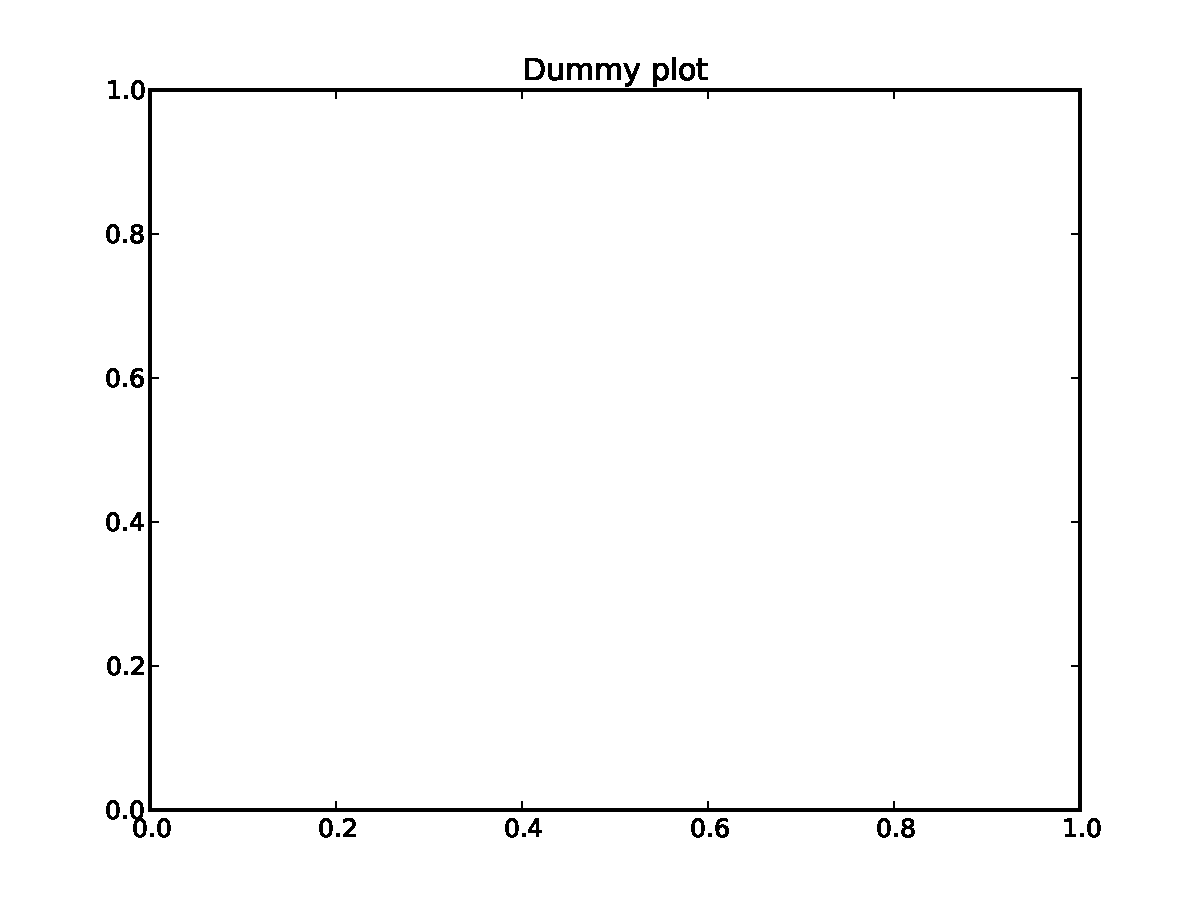
\includegraphics[width = 0.5\textwidth]{figs/dummy.pdf}
\label{fig:dpinitk}}
\subfloat[б)]{
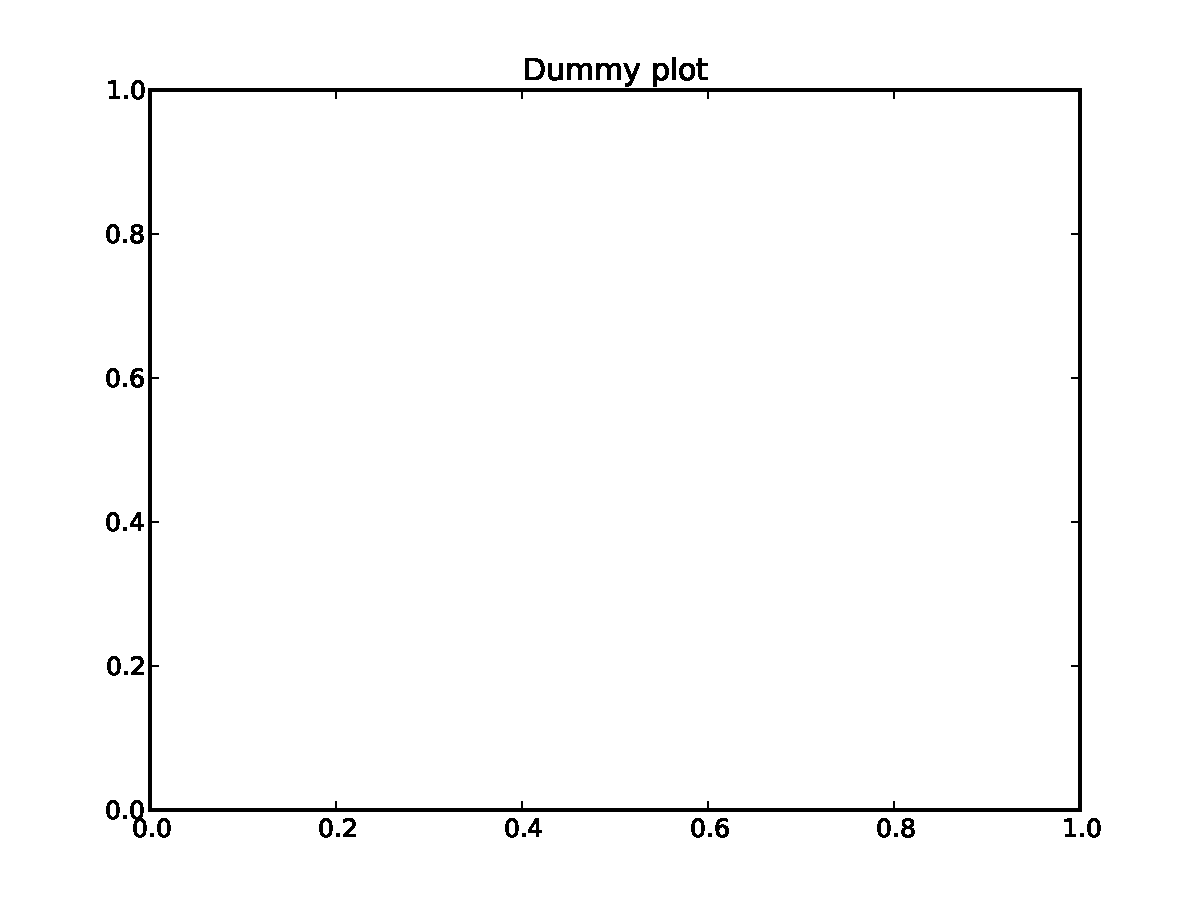
\includegraphics[width = 0.5\textwidth]{figs/dummy.pdf}
\label{fig:gpinita}}
\newline
\subfloat[в)]{
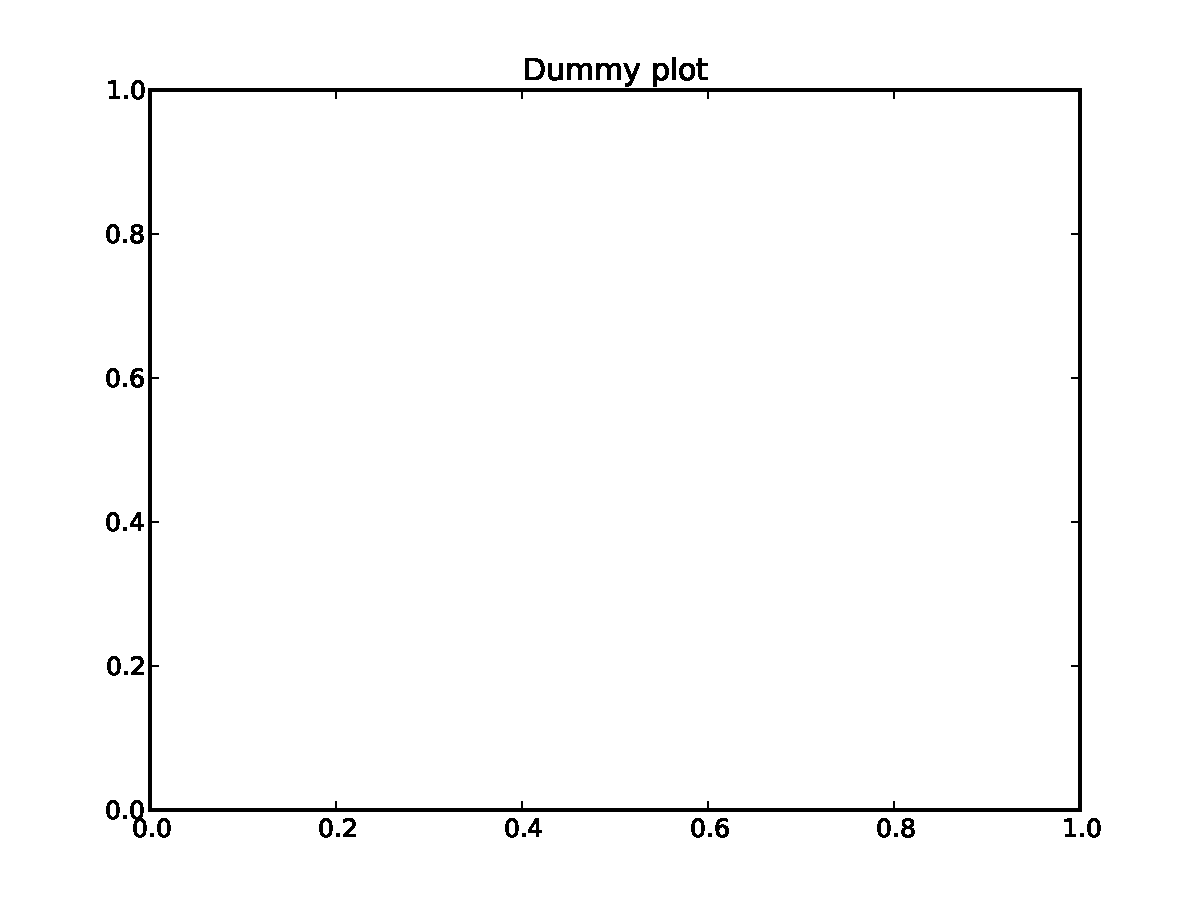
\includegraphics[width = 0.5\textwidth]{figs/dummy.pdf}
\label{fig:gpinitcpt}}
\newline
\caption{Результаты вычислений для $g= -1.241$, $p_{icp}= -0.088$, $p_{cp}=-0.137$:
\newlineа) для волнового числа; 
\newlineб) для амплитуды ПП;
\newlineв) для скачка теплоемкости, отнесенного к температуре.}
\end{figure}


\section{Обсуждение результатов}\label{sec:discuss}

В данном разделе проведен сравнительный анализ нелинейной \eqref{eq:snmodel} и одногармонической \eqref{eq:sinmodel} моделей распределения поля ПП в НСФ собственного СЭ Sn$_2$P$_2$Se$_6$. Результаты расчетов показывают, что предложенная sn-модель \eqref{eq:snmodel} более корректно описывает температурное поведение основных термодинамических характеристик НСФ в Sn$_2$P$_2$Se$_6$, в частности, вблизи точки фазового перехода в СФ. Так, в sn-модели \eqref{eq:snmodel} качественно правильно воспроизводится ход температурной зависимости волнового вектора волны модуляции ПП.
Данное исследование является первым этапом термодинамического анализа свойств НСФ в Sn$_2$P$_2$Se$_6$ Далее требуется определить значения материальных параметров для предложенной sn-модели \eqref{eq:snmodel}. Из анализа оценочной вариации материальных параметров следует, что при дальнейшем исследовании модели \eqref{eq:snmodel} и нахождении ее собственных значений материальных параметров особое внимание следует уделить области $g < -1.241,\, p_{icp} < -0.137$.
